\refstepcounter{Exercise}
\clearpage\subsection*{2−3 \theExercise 友だちのホームページを見てみよう}
\addtocounter{Exercise}{-1}\refstepcounter{Exercise}\label{friend}
% \clearpage\subsection*{2−3友だちのホームページを見てみよう}

\centering
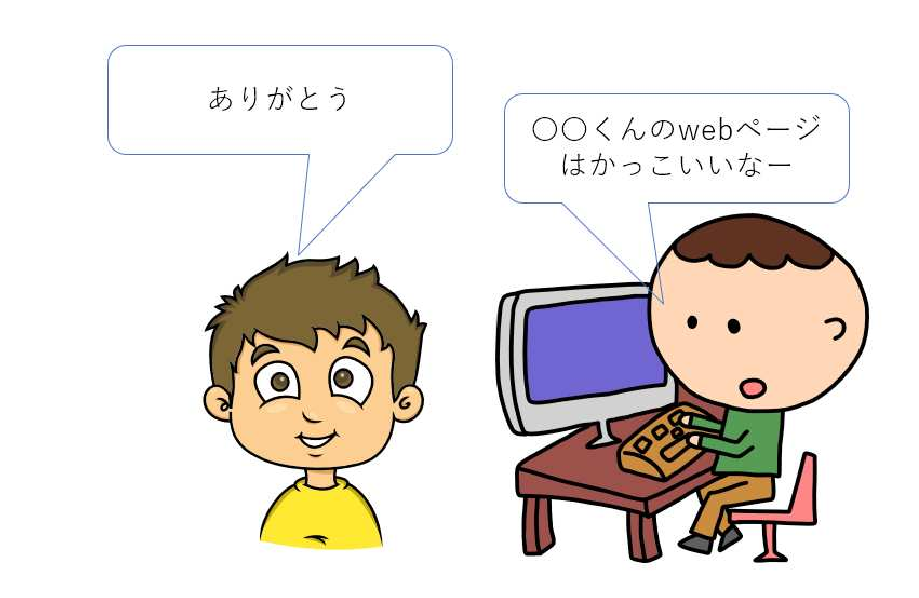
\includegraphics[width=10.423cm]{text07-img/ome7-img042}
\flushleft


\bigskip



1.
\ruby{左隣}{ひだりどなり}の友達のIPアドレスを確認しよう。

\ \ 友達のターミナルで次のコマンドをうってもらいましょう。

\ \ hostname -I

\ \ そのIPアドレスをメモしましょう。

\ \ [\underline{    }さんのIP:\underline{              }]


\bigskip

2.友達のウェブページを見て見ましょう。

\ \ 自分のサーバーを見るときは

\ \  \url{http://localhost:3000/}

\ \ でした。localhostというのが自分のサーバーという意味でした。

\ \ 今回は友達のサーバーを見たいのでlocalhostの代わりに友達のIPアドレスを打ちましょう。

\ \  \url{http://xxx.xxx.xxx.xxx:3000/}

\ \ \  \url{http://xxx.xxx.xxx.xxx:3000/index.html}

\ \ をブラウザのアドレスバーに打ってみましょう。

\ \ もし左隣の友達のIPアドレスが192.162.33.5だったら

\ \  \url{http://192.162.33.5:3000/index.html}

\ \ となります。

\ \ 友達のウェブページが表示されたら成功です!


\bigskip


\centering
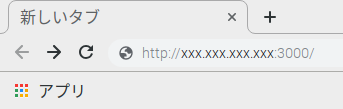
\includegraphics[width=10.659cm]{text07-img/ome7-img043.png}
\flushleft

\clearpage\subsection*{\bfseries
	注意}

	例題7-6の友達のホームページを見てみようでは、以下の図のように同じルータにつながっているラズベリーパイが公開しているホームページは、見ることができます。\ruby{基本}{きほん}同じグループの子たちのホームページは見れるので確認してみてください。

\centering
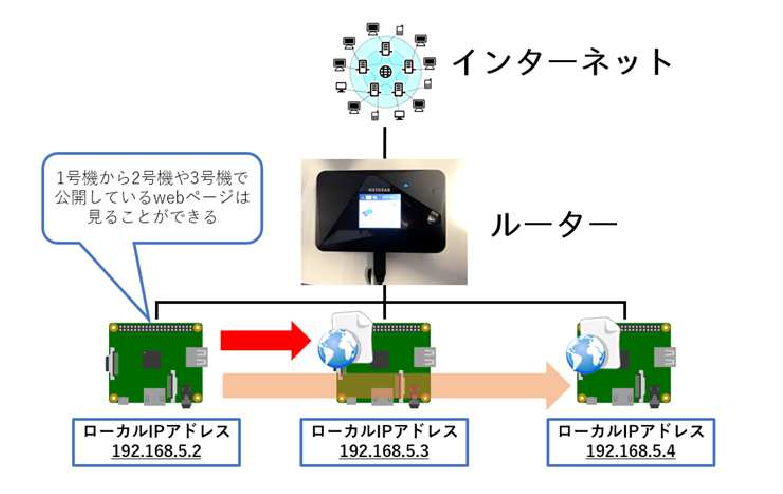
\includegraphics[width=0.75\textwidth]{text07-img/ome7-img044}
\flushleft


\bigskip



あと、他のルータに接続しているラズベリーパイが公開しているホームページは今回みることができません。実際に試してみても面白いと思います。


\bigskip

\centering
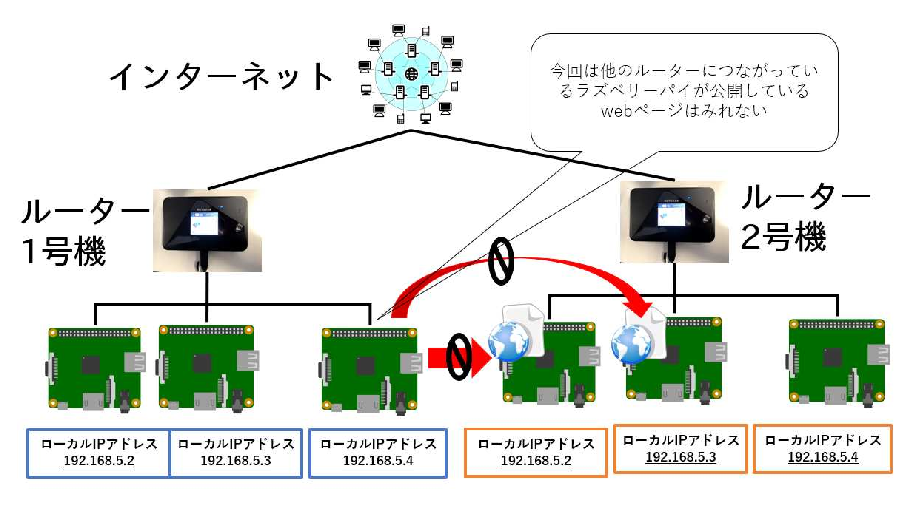
\includegraphics[width=0.75\textwidth]{text07-img/ome7-img045}
\flushleft


\bigskip

\refstepcounter{Question}\theQuestion 他のグループの友達のホームページを見てみよう、自分とは違うWi-Fiルータに接続している友達のホームページは見れたかどうか答えに書こう\label{Q:otherHP}\\
% 問題7-8  
% 他のグループの友達のホームページを見てみよう、自分とは違うWi-Fiルータに接続している友達のホームページは見れたかどうか答えに書こう


{\bfseries 
    \underline{答え:                           }
}


\bigskip

% \if0


% 	参考 接続できるネットワーク(Wi-Fiルータ)

% 	NTGR-4643\ \ \ \ パスワード 33995460

% 	NTGR-3EBC\ \ \ \ パスワード 34986626

% 	NTGR-3DFC\ \ \ \ パスワード 36976828

% \fi

\bigskip


\bigskip